\chapter{Advanced Construction Algorithms for SSA
   \Author{D.~Das \andAuthor U.~Ramakrishna \andAuthor V.~Sreedhar}}
%\chapter{Alternative SSA construction algorithms
\label{chapter:alternative_ssa_construction_algorithms}
\inputpath{part1}{alternative_ssa_construction_algorithms}
\inputprogress

{

\def\p{$\phi$}
\def\st#1{\rlap{\raisebox{3.4pt}{\kern3pt{\scriptsize\it #1}}}{\rightarrow}}
\def\stplus{\rlap{\raisebox{3.4pt}{\kern3pt{\scriptsize+}}}{\rightarrow}}
\def\St#1{\rlap{\raisebox{3.4pt}{\kern3pt{\scriptsize\it #1}}}{\Rightarrow}}
\def\depth{\textrm{depth}}
\newcommand\subtree[1]{\textsf{subtree}(#1)}

\def\p{$\phi$}
\def\iDFfwd{\iDF\!\!_{\textit{fwd}}}


\section{Introduction}

%FAB: Removed the mention of Cytron, Sreedhar etc. Replaced by more descriptive naming of the presented techniques
The placement of $\phi$-functions is an important step in the construction of Static Single Assignment (SSA) form. 
In SSA form every variable is assigned only once. 
At control-flow merge points \phifuns are added to ensure that every use of a variable corresponds to exactly one definition. 
In the rest of this chapter we will present three different approaches for placing \phifuns at appropriate merge nodes. 
Recall that SSA construction falls into two phases of $\phi$-placement and variable renaming. 
Here we present different approaches for the first phase for minimal SSA form.  
We first present some properties of the \DJ-graph\index{DJ-graph@\DJ-graph} 
that allow to compute the iterated dominance frontier of a given set of nodes 
$S$ by traversing the \DJ-graph from leafs to root.  \phifuns can then be 
placed using the \iDF set.
Based on the same properties, we then present an alternative scheme for computing \iDF-graph based on data-flow equations, this time using a traversal of the \DJ-graph from root to leafs. 
Finally we describe another approach for computing the iterated dominance frontier based on the loop nesting forest.



\section{Basic Algorithm}
\label{section:alternative_ssa_construction_algorithms:cytron}
We start by recalling the basic algorithm already described in~\ref{chapter:classical_construction_algorithm}. 
The original algorithm for placing \phifuns is based on computing the dominance frontier (\DF) set for the given control-flow graph. 
The dominance frontier\index{dominance frontier} $\DF(x)$ of a node $x$ is the set of all nodes $z$ such that $x$ dominates a predecessor of $z$, without strictly dominating $z$. 
%Too vague: removed
%Thus, from the point of view of $x$, the \DF nodes are the earliest appearance of paths joining the flow without passing through $x$.
For example, $\DF(8)= \{ 6, 8 \}$ in Figure~\ref{fig:cfg}. 
%FAB: Removed the mentions of complexity as the problem is not clearly stated (cost for the placement for one variable, for all...)
The basic algorithm for the placement of \phifuns consists in computing the 
iterated dominance frontier (\iDF) for a set of all definition points (or nodes 
where variables are defined).  Let $\Defs{v}$ be the set of nodes where 
variable $v$ is defined.  Given that the dominance frontier for a set of nodes 
is just the union of the \DF set of each node, we can compute $\iDF(\Defs{v})$ 
as a limit of the following recurrence equation (where $S$ is initially 
$\Defs{v}$):
\begin{eqnarray*}
\iDF_1(S) &=& \DF(S) \\
\iDF_{i+1} (S) &=& \DF(S \cup \iDF_i(S)) 
\end{eqnarray*}
A \phifun is then placed at each merge node in the  $\iDF(\Defs{v})$ set. 

\section{Computation of $\iDF(S)$ using \DJ-graphs}
\label{section:alternative_ssa_construction_algorithms:sreedhar}
We now present a linear time algorithm for computing the $\iDF(S)$ set of
a given set of nodes $S$ without the need for explicitly pre-computing the full 
\DF set.  The algorithm uses the \DJ-graph (see 
Chapter~\ref{chap:classical_construction_algorithm},
Section~\ref{sec:classical_construction_algorithm:phiinsertion} and 
Figure~\ref{fig:classical_construction_algorithm:iDF-J}) representation of 
a CFG.  The \DJ-graph for our example CFG is also shown in 
Figure~\ref{sub:alt:DJ}.  Rather than explicitly computing the \DF set, this 
algorithm uses a \DJ-graph to compute the $\iDF(\Defs{v})$ on the fly. 

\subsection{Key Observations} 
 
Now let us try to understand how to compute the \DF set for a \emph{single node} using the \DJ-graph.
%FAB: add key observation that J-edge is going up (important to understand the other key observation)
%FAB: replaced level by depth (to disambiguate between low level / high in the figure)
Consider the \DJ-graph shown in Figure~\ref{sub:alt:DJ} where the depth of 
a node is the  distance from the root in the dominator tree.
The first key observation is that a \DF-edge never goes down to a greater depth.
To give a raw intuition of why this property holds, suppose there were 
a \DF-edge from 
8 to 7, then there would be a path from 3 to 7 through 
  8 without flowing through 6, which contradicts the dominance of 7 by 6. 


As a consequence, to compute $\DF(8)$ we can simply walk down the dominator (D) tree from node 8 and from each visited node $y$, identify all join (J) edges $y \st{J} z$ such that $z.\depth \leq 8.\depth$. 
For our example the J-edges that satisfy this condition are $10 \st{J} 8$ and $9 \st{J} 6$. 
Therefore $\DF(8) = \{6, 8\}$. 
To generalize the example, we can compute the \DF of a node $x$ using the following formula (see Figure \ref{fig:alt:exemple-1-df} for a illustration):
$$\DF(x) = \{z\mid\exists\, y\in\dominated{x} \; \wedge \; y \st{J} z \in \textrm{J-edges} \; \wedge \; z.\depth \leq x.\depth \}$$
where 
$$\dominated{x} = \{ y\mid x\dom y \}$$


\begin{figure}[htb]
  % \centerline{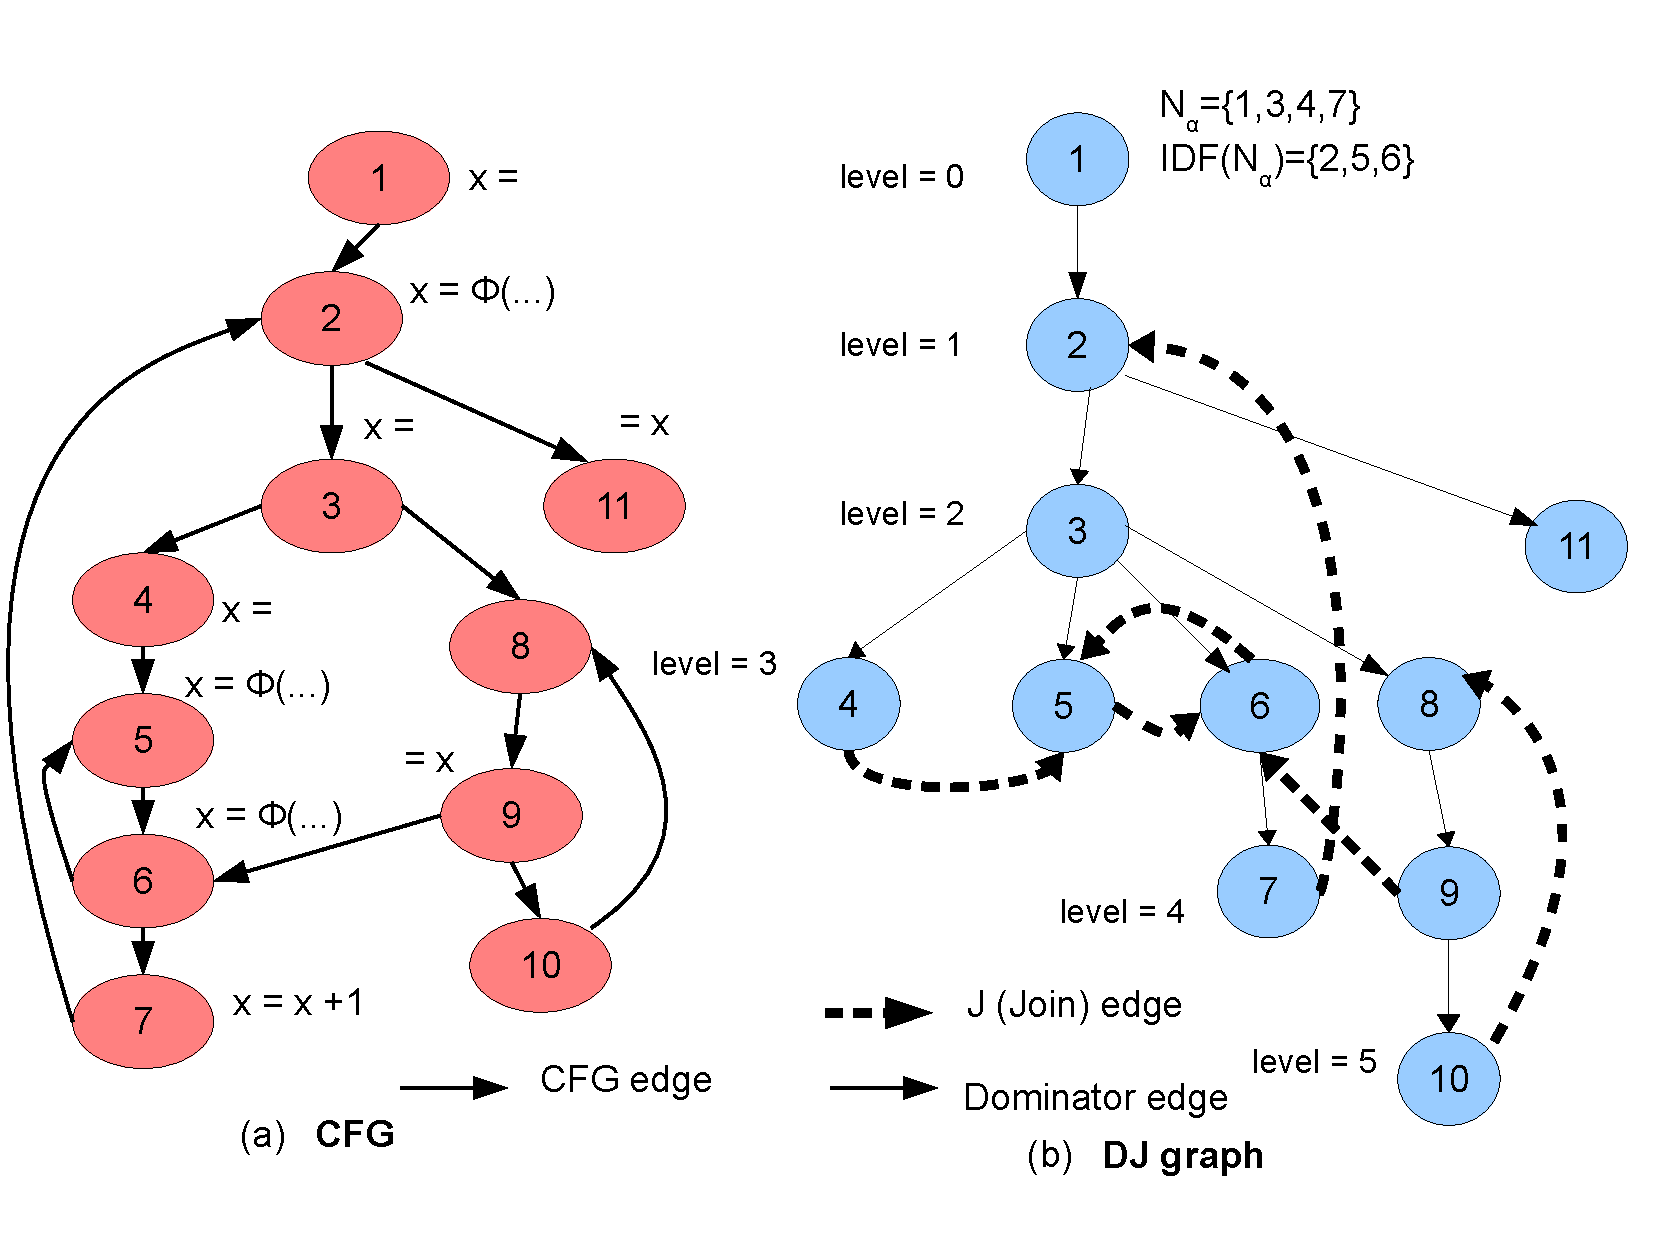
\includegraphics[scale=0.4]{cfglive_new.pdf}}
  \subfloat[][CFG]{
    \tikzfigure{cfglive}
    \label{sub:alt:cfg}
  }
  \subfloat[][\DJ-graph]{
    \tikzsubfigure[1]{cfgdj}
    \label{sub:alt:DJ}
  }
  \caption{A motivating example.}
  \label{fig:cfg}
\end{figure} 

Now we can extend the above idea to compute the \iDF for \emph{a set of nodes}, and hence the placement of \phifuns. 
This algorithm does not precompute \DF; 
given a set of initial nodes $S=\Defs{v}$ for which we want to compute the relevant set of \phifuns, a key observation can be made. 
Let $w$ be an ancestor node of a node $x$ on the dominator tree. 
If $\DF(x)$ has already been computed before the computation of $\DF(w)$, the traversal of $\dominated{x}$ can be avoided and $\DF(x)$ directly used for the computation of $\DF(w)$. 
This is because nodes reachable from $\dominated{x}$ are already in $\DF(x)$. 
However, the converse may not be true, and therefore the order of the computation of \DF is crucial.

To illustrate the key observation consider the example \DJ-graph in 
Figure~\ref{sub:alt:DJ}, and let us compute $\iDF(\{3,8\})$.  It is clear from 
the recursive definition of \iDF that we have to compute $\DF(3)$ and $\DF(8)$ 
as a first step.  Now supposing we start with node $3$ and compute $\DF(3)$.  
The resulting \DF set is $\DF(3) = \{2\}$.  Now supposing we next compute the 
\DF set for node $8$, and the resulting set is $\DF(8) = \{6,8\}$.  Notice here 
that we have already visited node $8$ and its sub-tree when visiting node $3$.  
We can avoid such duplicate visits by ordering the computation of \DF set so 
that we first compute $\DF(8)$ and then during the computation of $\DF(3)$ we 
avoid visiting the sub-tree of node $8$, and use the result $\DF(8)$ that was 
previously computed.

Thus, to compute $\DF(w)$, where $w$ is an ancestor of $x$ in the \DJ-graph, we do not need to compute it from scratch as we can re-use the information computed as part of $\DF(x)$ as shown. 
For this, we need to compute the \DF of deeper (based on depth) nodes (here, $x$), before computing the \DF of a shallower node (here, $w$). The formula is as follows, with Figure~\ref{fig:alt:exemple-2-df} illustrating the positions of nodes $z$ and $z'$.

\begin{flalign*}
\DF(w) = & \left\{z \mid z \in \DF(x) \wedge z.\depth \leq w.\depth\right\} \ \cup  \\
          &  \left\{z' \mid y \in \subtree{w} \setminus \subtree{x} \wedge y \st{J} z' 
          \wedge z'.\depth \leq w.\depth \right\}
%}. 
\end{flalign*}


\begin{figure}[t]
  \subfloat[][]{
    \tikzsubfigure[1]{example-df}
    \label{fig:alt:exemple-1-df}
  }
  \subfloat[]{
    \tikzsubfigure[2]{example-df}
    \label{fig:alt:exemple-2-df}
  }
  \caption{Illustrating examples to the $\DF$ formulas.}
\end{figure}



\subsection{Main Algorithm}
\def\bucket{\textit{OrderedBucket}\xspace}
\def\insertN{\textrm{InsertNode}}
\def\getN{\textrm{GetDeepestNode}()}
\def\visited{\textrm{visited}}

In this section we present the algorithm for computing \iDF. 
Let, for node $x$, $x.\depth$ be its depth from the root node $r$, with $r.\depth= 0$. 
To ensure that the nodes are processed according to the above observation we use a simple array of sets \bucket, and two functions defined over this array of sets: 
(1) $\insertN(n)$ that inserts the node $n$ in the set $\bucket[n.\depth]$, and (2) \getN\ that returns a node from the \bucket with the deepest depth number.

\begin{algorithm}
  \caption{Algorithm for computing $\iDF(S)$ set.}
  \label{algo:IDFMain}

  \KwIn{\DJ-graph representation of a program}
  \KwIn{$S$: set of CFG nodes}
  \KwOut{$\iDF(S)$}

  $\iDF \gets \emptyset$\;
  \ForEach{node $x \in S $}{
    $\insertN(x)$\;
    $x.\visited \gets \false $\;
  }
  \While(\Comment*[f]{Get node from the deepest depth}){$x \gets 
  \getN$}{  \label{C:get} $\textit{current\_x} \gets x$\;
    $x.\visited \gets \true$\;
    Visit($x$)\Comment*[r]{Find $\DF(x)$}
  }
  \textbf{return} \iDF
\end{algorithm}

%FAB: was on CFG. Made it on DJ-graph as explained in the text
\begin{procedure}
  \caption{Visit($y$)}
  \label{proc:visit}
  \ForEach{J-edge $y \st{J} z$}{
    \If{$z.\depth \leq \textit{current\_x}.\depth$}{
      \If{$z \not \in \iDF$}{
        $\iDF \gets \iDF \cup \{z\}$\;   \label{line:alt:idf}
        \lIf{$z \not  \in S$}{
          $\insertN(z)$ \label{C:insert}
        }
      }
    }
  }
  \ForEach{D-edge $y \st{D} y'$}{  
    \If{$y'.\textit{visited} = \false $}{
      $y'.\visited \gets \true$\;
      \tcc{if($y'.\textit{boundary} = \false$)   \label{C:cached} 
    \hfill$\rhd$ See the section on Further Reading for details}
      Visit($y'$) \label{C:dedges}
    }
  }
\end{procedure}

In Algorithm~\ref{algo:IDFMain}, at first we insert all nodes belonging to $S$ in the \textit{OrderedBucket}. 
Then the nodes are processed in a bottom-up fashion over the \DJ-graph from deepest node depth to least node depth by calling \ref{proc:visit}($x$). 
The procedure \ref{proc:visit}($x$) essentially walks top-down in the \DJ-graph avoiding already visited nodes. 
During this traversal it also peeks at destination nodes of J-edges.  Whenever 
it notices that the depth number of the destination node of a J-edge is less 
than or equal to the depth number of the $\textit{current\_x}$, the destination 
node is added to the $\iDF$ set (Line~\ref{line:alt:idf}) if it is not present 
in \iDF already.  Notice that at Line~\ref{C:insert} the destination node is 
also inserted in the {\it OrderedBucket} if it was never inserted before.  
Finally at Line~\ref{C:dedges} we continue to process the nodes in the sub-tree 
by visiting over the D-edges.  When the algorithm terminates, the set $\iDF$ 
contains the iterated dominance frontier for the initial set $S$.

\begin{figure}[htb]
    % \centerline{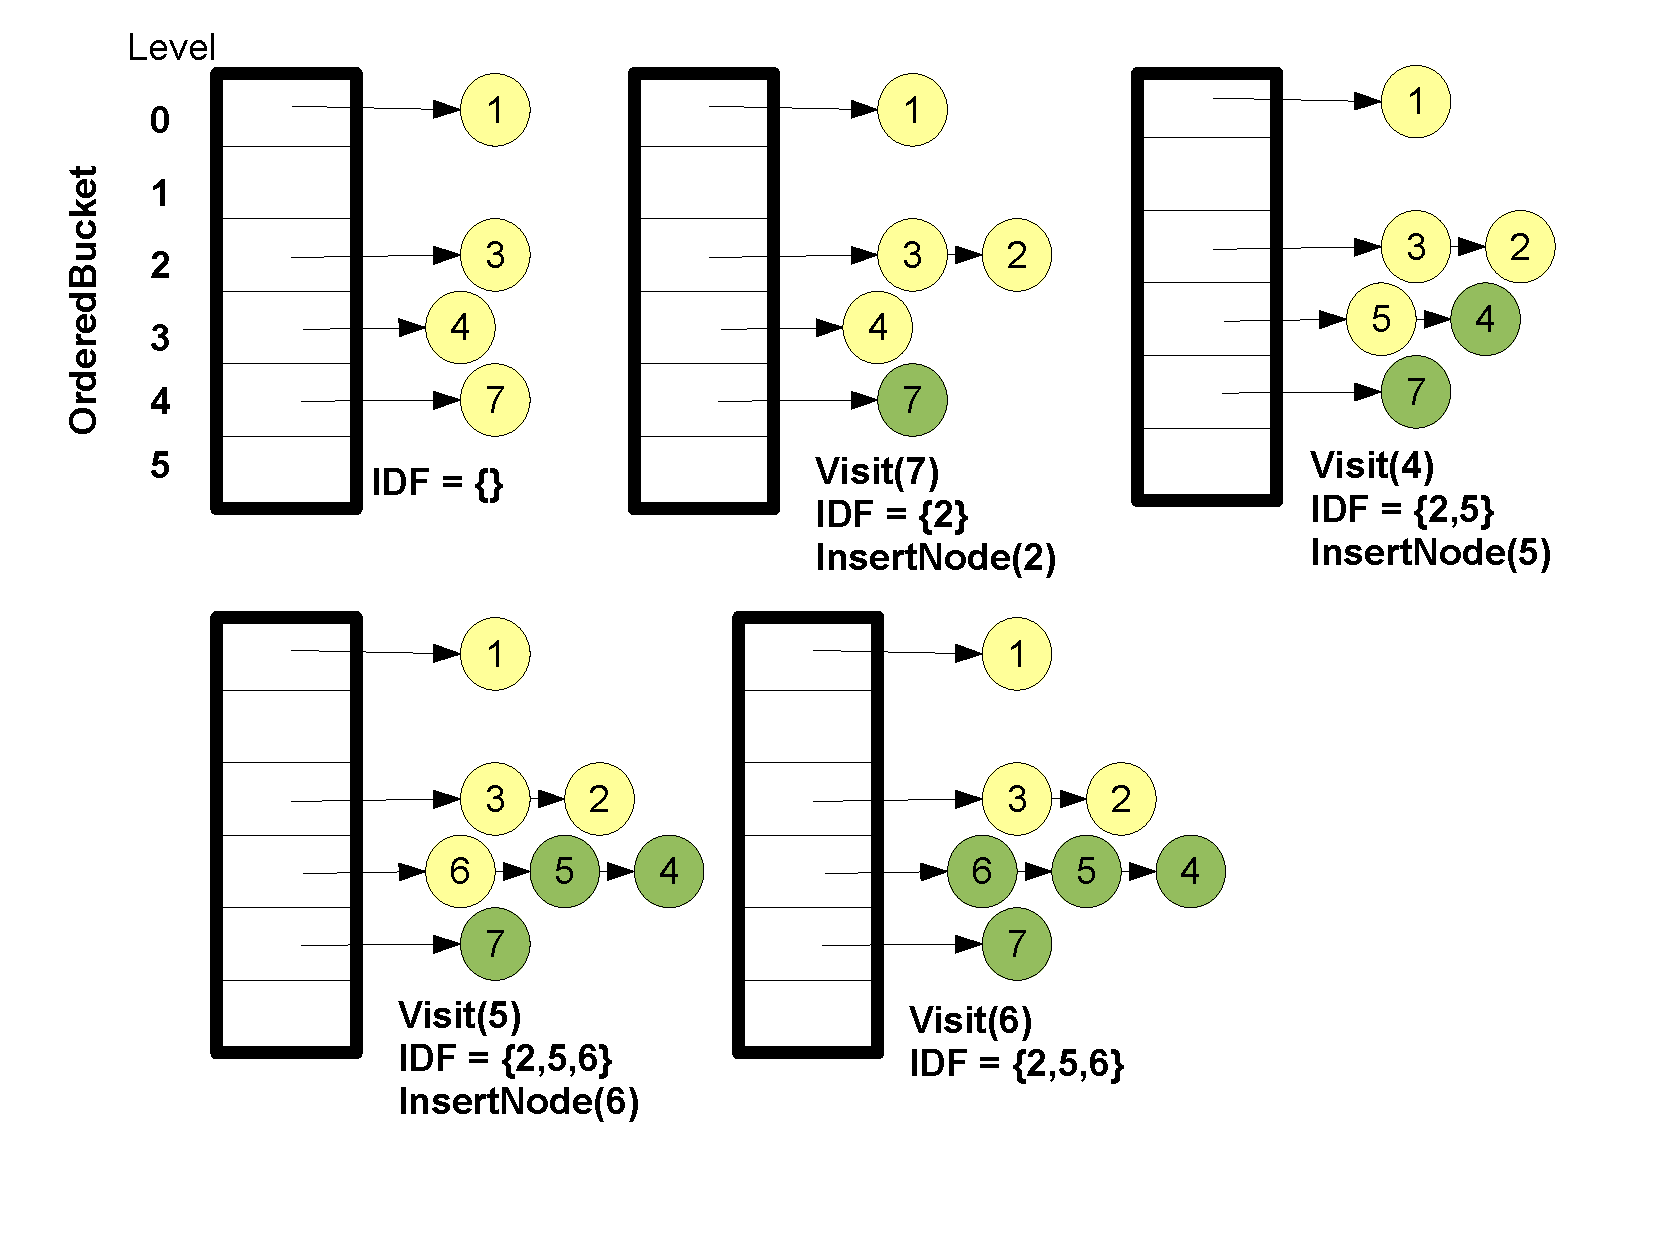
\includegraphics[scale=0.3]{sreedhargao.pdf}}
    \centerline{\tikzfigure{sreedhargao}}
    \caption{Phases of Algorithm~\ref{algo:IDFMain} for $S=\Defs{v}=\{1,3,4,7\}$.}
    \label{fig:sreedhargao}
    \end{figure} 


In Figure~\ref{fig:sreedhargao}, some of the phases of the algorithm are depicted for clarity. 
The \textit{OrderedBucket} is populated with the nodes $1,3,4$ and $7$ corresponding to $S=\Defs{v}=\{1,3,4,7\}$. 
The nodes are placed in the buckets corresponding to the depths at which they appear. 
Hence, node~1 which appears at depth~0 is in the 0-th bucket, node~3 is in bucket~2 and so on. 
Since the nodes are processed bottom-up, the first node that is visited is node~7. 
The J-edge $7 \st{J} 2$ is considered, and the $\iDF$ set is empty: the $\iDF$ 
set is updated to hold node~2 according to Line~\ref{line:alt:idf} of the Visit 
procedure.  In addition, $\insertN(2)$ is invoked and node~2 is placed in 
bucket~2.  The next node visited is node~4.  The J-edge $4 \st{J} 5$ is 
considered which results in the new $\iDF = \{2,5\}$.  The final $\iDF$ set 
converges to $\{2,5,6\}$ when node~5 is visited.  Subsequent visits of other 
nodes do not add anything to the $\iDF$ set.  An interesting case arises when 
node~3 is visited.  Node~3 finally causes nodes 8, 9 and 10 also to be visited 
(Line~\ref{C:dedges} during the down traversal of the D-graph).  However, when 
node~10 is visited, considering J-edge $10 \st{J} 8$ does not result in an 
update of the $\iDF$ set as the depth of node~8 is deeper than that of node~3.


\section{Data-flow computation of \iDF-graph using \DJ-graph}
%FAB: removed all the stuff on merge set as:
%    M(S)=iDF(S)
%    The algorithm is nothing else than: computation of DF using a traversal of J-edges & walking up D-edges (standard algorithm); computation of iDF by transitive closure

In this section we describe a method to iteratively compute the \iDF~relation using a data-flow formulation. 
As already mentioned, the \iDF relation can be computed using a transitive closure of the \DF-graph, which in turn can be computed from the \DJ-graph. 
In the algorithm proposed here, explicit \DF-graph construction or the transitive closure formation are not necessary. 
Instead, the same result can be achieved by formulating the $\iDF$ relation as a data-flow problem and solving it iteratively. 
For several applications, this approach has been found to be a fast and effective method to construct $\iDF(x)$ for each node $x$ and the corresponding \phifun placement using the $\iDF(x)$ sets.

%FAB: highlighted the data-flow equation
\begin{center}
  \textbf{Data-flow equation:}\\
  {\it 
  Consider a J-edge $y \st{J} z$.\\
  Then for all nodes $x$ such that $x$ dominates $y$ and $x.\depth \geq z.\depth$:
  $$\iDF(x) = \iDF(x) \cup \iDF(z) \cup \{z\}$$}
\end{center}

The set of data-flow equations for each node $n$ in the \DJ-graph can be solved iteratively using a top-down pass over the \DJ-graph. 
To check whether multiple-passes are required over the \DJ-graph before a fixed-point is reached for the data-flow equations, we devise an ``inconsistency condition'' stated as follows:

%\paragraph{Inconsistency Condition:}
\begin{center}
\bf{Inconsistency Condition:}\\
\it{For a J-edge, $y' \st{J} x$, if $y'$ does not satisfy
$\iDF(y')\supseteq \iDF(x)$,\\ then the node $y'$ is said to be inconsistent}. 
\end{center}

The algorithm described in the next section is directly based on the method of building up the $\iDF(x)$ sets of the nodes as each J-edge is encountered in an iterative fashion by traversing the \DJ-graph top-down. 
If no node is found to be \emph{inconsistent} after a single top-down pass, all the nodes are supposed to have reached fixed-point solutions. 
If some node is found to be inconsistent, multiple passes are required until a fixed-point solution is reached.


\subsection{Top Down \iDF Set Computation}

\begin{procedure}
  \caption{TDMSCMain()}
  \label{proc:tdmscmain}
  \KwIn{A \DJ-graph representation of a program.}
  \KwOut{The \iDF sets for the nodes.}
  \ForEach{node $x \in$ \DJ-graph}{
    $\iDF(x) \gets \{\}$
  }
  \lRepeat{TDMSC-I(\DJ-graph)}{}
\end{procedure}

\begin{function}
  \caption{TDMSC-I(\DJ-graph)}
  \label{proc:alt:tdmscI}
  $\textit{RequireAnotherPass} \gets \false$\;

  \lForEach{edge $e$}{
    $e.\visited \gets \false$
  }
  \While{$z \gets$ next node in B(readth) F(irst) S(earch) order of \DJ-graph}{ 
    \label{line:alt:bfs}
    \ForEach{incoming edge $e = y \st{J} z$}{ \label{line:alt:jedge}
      \If{not $e.\visited$}{
        $e.\visited \gets \true$\;
        $x \gets y$\;
              % $\textit{lx} = \nullprog$; %FAB: removed: not necessary
        \While{$(x.\depth\ge z.\depth)$}{
          \label{line:alt:mwhiles}
          $\iDF(x) \gets \iDF(x)\cup \iDF(z)\cup \{z\}$\;
          $\textit{lx} \gets x$\;
          $x \gets \textrm{parent}(x)$ \Comment*{dominator tree 
          parent}
        }
        \ForEach{incoming edge $e' = y^{'} \st{J} \textit{lx}$}{
          \label{line:alt:lnode}
          \If{$e'.\visited$}{
            \If(\Comment*[f]{Check inconsistency}){$\iDF(y') 
              \not\supseteq \iDF(\textit{lx})$}{%
                 $\textit{RequireAnotherPass} \gets \true$;
            }
          }
        }
      }
    }
  }
  \Return{$\textit{RequireAnotherPass}$}
\end{function}

%==
%\begin{figure}[!ht]
%\centering
%\begin{minipage}[t]{5in}
%\noindent{\bf Input:} A \DJ-graph representation of a program.
%\noindent{\bf Output:} The \iDF sets for the nodes.
%
%\setcounter{linectr}{0}
%Procedure TDMSCMain
%\{
%\begin{code}
%\x1 $\forall$ node $x \in$ \DJ-graph set $\iDF(x) = \{\}$
%\x1 {\it done = false};
%\x1 {\bf while} (! {\it done}) {\bf do}
%\x2     {\it done} = TDMSC-I(\DJ-graph);
%\x1 {\bf end while}
%\end{code}
%\}
%
%%FAB: Added initialization of visited 
%Procedure TDMSC-I(\DJ-graph)
%\{
%\begin{code}
%%\textbf{Algorithm: Top Down Merge Set Computation (TDMSC-I)}
%%Input: $\DJ$-graph
%%Outputs: Complete Merge Sets for every node of the \DJ-graph
%
%\x1 $\textit{RequireAnotherPass}=\false$;
%\x1 {\bf for} ($\forall$ edge $e$) {\bf do} $e.\visited = \false$;
%
%\x1 {\bf while} ($z$ = next node in B(readth) F(irst) S(earch) order of \DJ-graph) {\bf do} \label{C:bfs}
%%\x2      $z$ $=$ Next Node in BFS list
%\x2      {\bf for} ($\forall$ incoming edge $e = y \st{J} z$) {\bf do} \label{C:jedge}
%\x3          {\bf if} ($e.\visited=\false$) {\bf then}
%\x4              $e.\visited=\true$;
%\x4              $\textit{x} = y$;
%%\x4              $\textit{lx} = \nullprog$; %FAB: removed: not necessary
%\x4              {\bf while} $(x.\depth\ge z.\depth)$ {\bf do} \label{C:mwhiles}
%
%\x5                   $\iDF(x)=\iDF(x)\cup \iDF(z)\cup \{z\}$;
%\x5                   $\textit{lx}=x$;
%\x5                   $x=\textrm{parent}(x)$; //dominator tree parent 
%\x4              {\bf end while} \label{C:mwhilee}
%\x4              {\bf for} ($\forall$ incoming edge  $e' = y^{'} \st{J} \textit{lx}$) {\bf do} \label{C:lnode}
%\x5                  {\bf if} ($e'.\visited=\true$) {\bf then}
%\x6                     {\bf if} $(\iDF(y') \not\supseteq \iDF(\textit{lx}))$ {\bf then} //Check inconsistency
%\x7                         $\textit{RequireAnotherPass} = \true$;
%\x6                     {\bf end if}
%\x5                  {\bf end if}
%\x4              {\bf end for}
%\x3          {\bf end if}
%\x2     {\bf end for}
%\x1 {\bf end while}
%\x1 {\bf return} $\textit{RequireAnotherPass}$;
%\end{code}
%\}
%\end{minipage}
%\caption{Top Down \iDF Set Computation.}
%\label{F:tdmsc}
%\end{figure} 

The first and direct variant of the approach laid out above is poetically 
termed \ref{proc:alt:tdmscI}.  This variant works by scanning the \DJ-graph in 
a top-down fashion as shown in Line~\ref{line:alt:bfs} of Function 
\ref{proc:alt:tdmscI}.
All $\iDF(x)$ sets are set to the empty set before the initial pass of 
\ref{proc:alt:tdmscI}.  The $\iDF(x)$ sets computed in a previous pass are 
carried over if a subsequent pass is required.

The \DJ-graph is visited depth by depth.
During this process, for each node $z$ encountered, if there is an \emph{incoming} J-edge $y \st{J} z$ as in Line~\ref{line:alt:jedge}, then a separate bottom-up pass starts at Line~\ref{line:alt:mwhiles} (see Figure~\ref{sub:alt:example-TDMSC} for a snapshot of the variables during algorithm execution).

\begin{figure}[b!]
  \subfloat[TDMSC-I snapshot]{
    \tikzfigure{example-TDMSC}
    \label{sub:alt:example-TDMSC}
  }
  \hfill
   \subfloat[][\DJ-graph]{
     \tikzsubfigure[2]{cfgdj}
    \label{sub:alt:DJbis}
  }

  \caption{\protect\subref{sub:alt:example-TDMSC} Snapshot during execution of the \ref{proc:alt:tdmscI} algorithm and \protect\subref{sub:alt:DJbis} Recall of running example.}
  \label{fig:alt:example-TDMSC}
\end{figure}



This bottom-up pass traverses all nodes $x$ such that $x$ dominates $y$ and $x.\depth \geq y.\depth$, updating the $\iDF(x)$ values using the aforementioned data-flow equation. 
Line~\ref{line:alt:lnode} is used for the inconsistency check. 
\textit{RequireAnotherPass} is set to \true only if a fixed point is not reached and the inconsistency check succeeds for some node.

There are some subtleties in the algorithm that should be noted. 
Line~\ref{line:alt:lnode} of the algorithm visits incoming edges to \textit{lx} only when \textit{lx} is at the same depth as $z$, which is the current depth of inspection and the incoming edges to \textit{lx}'s posterity are at a depth greater than that of node $z$ and are unvisited yet.



%FAB: Fixed running example that did not fit the algorithm
Here, we will briefly walk through TDMSC-I using the \DJ-graph of 
Figure~\ref{sub:alt:DJ} (reprinted here as \ref{sub:alt:DJbis}).  Moving top-down over the graph, the first J-edge 
encountered is when $z=2$, i.e., $7 \st{J} 2$.  As a result, a bottom-up climbing of the nodes 
happens, starting at node $7$ and ending at node $2$ and the \iDF sets of these 
nodes are updated so that $\iDF(7) = \iDF(6) = \iDF(3) = \iDF(2) = \{2\}$.  The 
next J-edge to be visited can be any of $5 \st{J} 6$, $9 \st{J} 6$, $6 \st{J} 
5$, $4 \st{J} 5$, or $10 \st{J} 8$ at $\depth = 3$.  Assume node 
6 is visited first, and thus it is $5 \st{J} 6$, followed by  $9 \st{J} 6$.
This results in $\iDF(5) = \iDF(5) \cup \iDF(6) \cup \{6\} = \{2,6\}$, $\iDF(9) = \iDF(9) \cup \iDF(6) \cup \{6\} = \{2,6\}$, and $\iDF(8) = \iDF(8) \cup \iDF(6) \cup \{6\} = \{2,6\}$.
Now, let $6 \st{J} 5$ be visited. 
Hence, $\iDF(6) = \iDF(6) \cup \iDF(5) \cup \{5\} = \{2,5,6\}$. 
At this point, the \emph{inconsistency check} comes into the picture for the edge $6 \st{J} 5$, as $5 \st{J} 6$ is another J-edge that is already visited and is an incoming edge of node $6$. 
Checking for $\iDF(5) \supseteq \iDF(6)$ fails, implying that the $\iDF(5)$ needs to be computed again. 
This will be done in a succeeding pass as suggested by the \textit{RequireAnotherPass} value of true. 
In a second iterative pass, the J-edges are visited in the same order. 
Now, when $5 \st{J} 6$ is visited, $\iDF(5) = \iDF(5) \cup \iDF(6) \cup \{6\} = \{2,5,6\}$ as this time $\iDF(5) = \{2,6\}$ and $\iDF(6) = \{2,5,6\}$. 
On a subsequent visit of $6 \st{J} 5$, $\iDF(6)$ is also set to $\{2,5,6\}$. 
The inconsistency does not appear any more and the algorithm proceeds to handle the edges $4 \st{J} 5$, $9 \st{J} 6$ and $10 \st{J} 8$ which have also been visited in the earlier pass. 
TDMSC-I is invoked repeatedly by a different function which calls it in a loop till \textit{RequireAnotherPass} is returned as \false as shown in the procedure TDMSCMain.

%\subsubsection { Final \phifun placement using Merge Sets }
Once the iterated dominance frontier relation is computed for the entire CFG, placing $\phi$ is a straightforward application of the $\iDF(x)$ values for a given $\Defs{x}$, as shown in Algorithm~\ref{proc:phi-placement}.


\begin{algorithm}
  \KwIn{A CFG with \iDF sets computed and $\Defs{x}$.}
  \KwOut{Blocks augmented by \phifuns for the given $\Defs{x}$.}
  \ForEach{$n \in \Defs{x}$} {
    \ForEach{$n' \in \iDF(n)$} {
      Add a $\phi$ for $n$ in $n^{'}$ if not placed already
    }
  }
  \caption{$\phi$-placement for $\Defs{x}$ using $\iDF$ sets.}
  \label{proc:phi-placement}

\end{algorithm}

% \begin{figure}[!ht]
% \centering
% \begin{minipage}[t]{5in}
  % \noindent{\bf Input:} A CFG with \iDF sets computed and $\Defs{x}$.
  % \noindent{\bf Output:} Blocks augmented by \phifuns for the given $\Defs{x}$.
%
% \setcounter{linectr}{0}
%
% Procedure $\phi$-placement for $\Defs{x}$
% \{
% \begin{code}
% \x1 {\bf for} ($\forall n \in \Defs{x}$) {\bf do}
% \x2   {\bf for} ($\forall n^{'} \in \iDF(n)$) {\bf do}
% \x3       Add a $\phi$ for $n$ in $n^{'}$ if not placed already
% \x2   {\bf end for}
% \x1 {\bf end for}
% \end{code}
% \}
% \end{minipage}
% \caption{$\phi$-placement using \iDF sets.}
% \label{F:phip}
% \end{figure} 


\section{Computing Iterated Dominance Frontier Using Loop Nesting Forests}
\label{section:alternative_ssa_construction_algorithms:loop}
This section illustrates the use of \emph{loop nesting forests} to construct 
the iterated dominance frontier (\iDF) of a set of vertices in a CFG. This 
method works with reducible as well as irreducible loops.


\subsection{Loop nesting forest}%
A loop nesting forest\index{loop nesting forest}
is a data structure that represents the loops in a CFG and the containment relation between them. 
In the example shown in Figure~\ref{sub:alt:lnf-cfg} the loops with back edges $11 \rightarrow 9$ and $12 \rightarrow 2$ are both reducible loops.
The corresponding loop nesting forest is shown in Figure~\ref{sub:alt:lnf-lnf} and consists of two loops whose header nodes are $2$ and $9$.
The loop with header node $2$ contains the loop with header node $9$.

    \begin{figure}[t]
    % \centerline{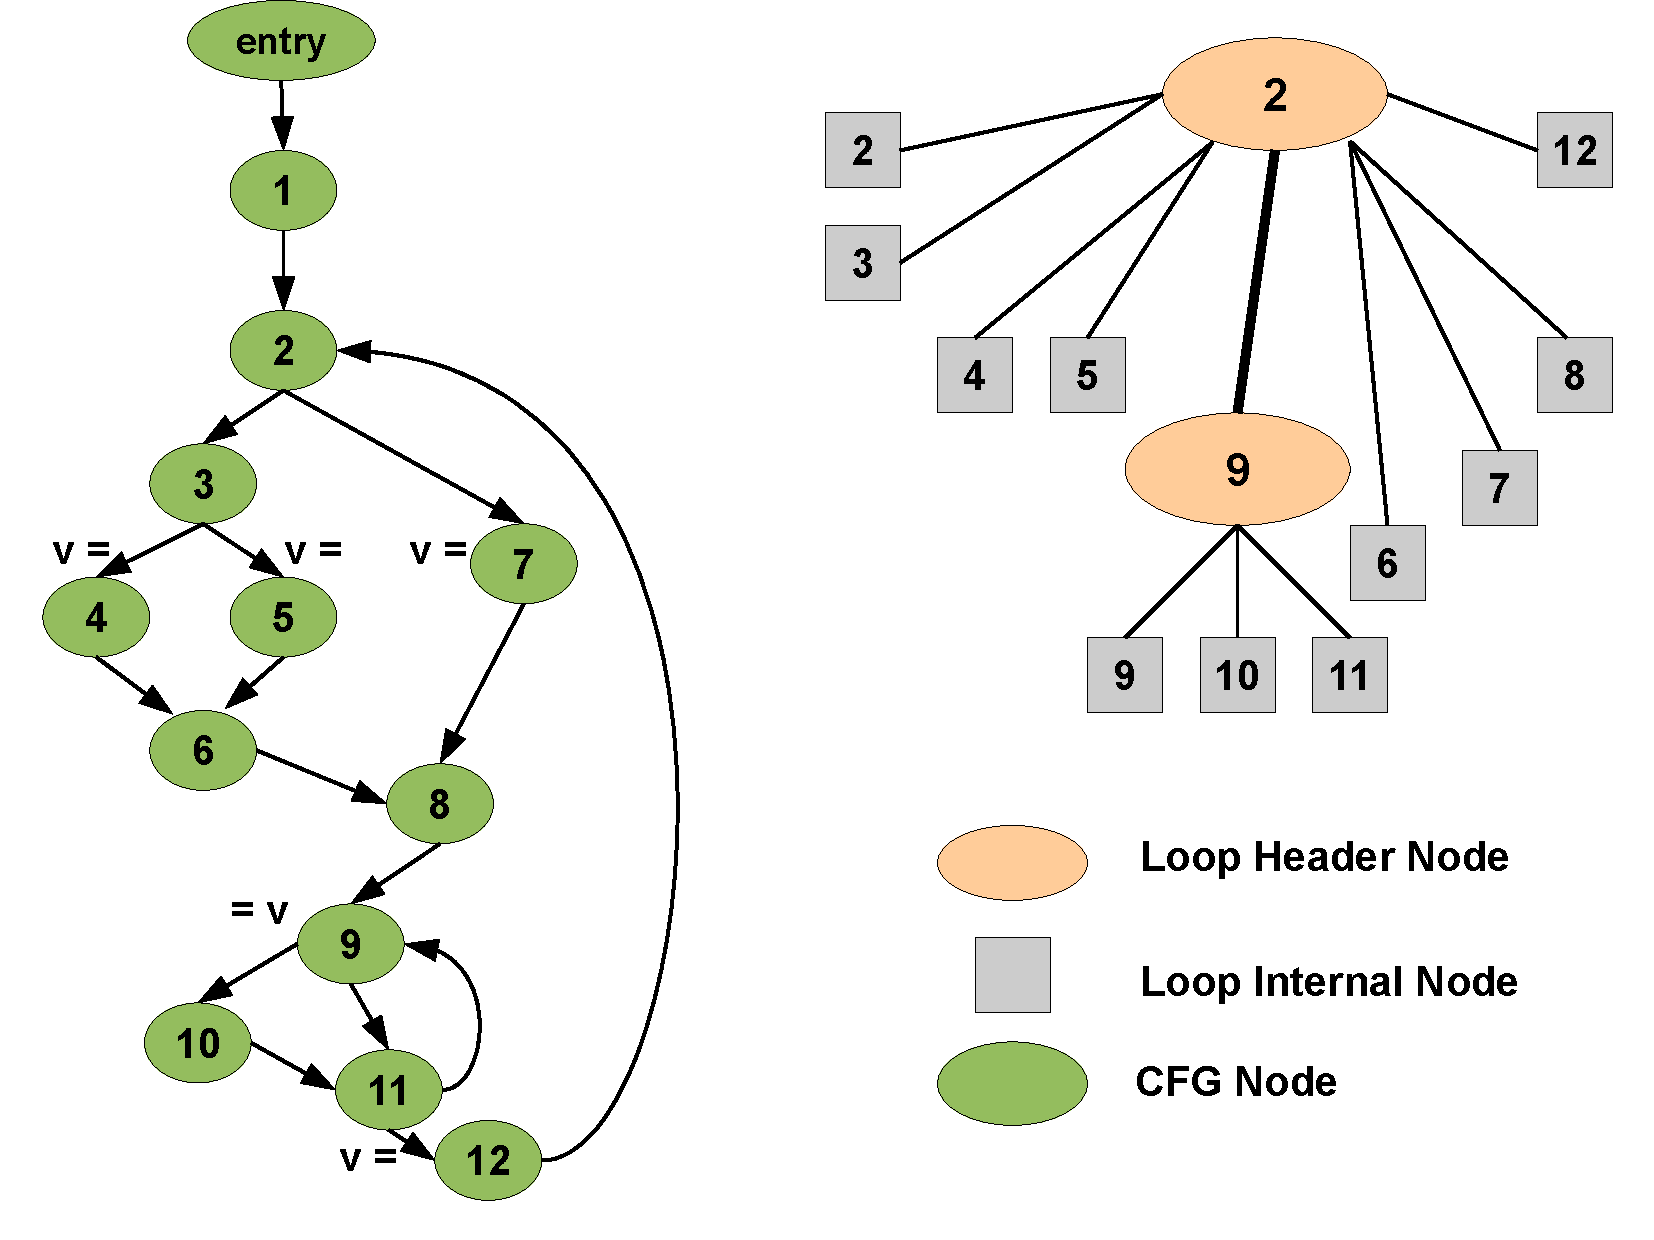
\includegraphics[scale=0.3]{lnfred.pdf}}
    \hfill
    \subfloat[CFG]{\tikzfigure{lnfcfg}\label{sub:alt:lnf-cfg}}
    \hfill
    % \qquad
    \subfloat[Loop Nesting Forest]{\tikzfigure{lnfred}\label{sub:alt:lnf-lnf}}
    \hfill\null
    \caption{An example CFG with four defs and one use of variable $v$ and its loop nesting forest.}
    \label{fig:lnf}
    \end{figure} 


\subsection{Main Algorithm}
%FAB: replaced acyclic graph by forward CFG & fixed minor corner cases
The idea is to use the forward CFG\index{forward control-flow graph}, an acyclic version of the control-flow graph (i.e., without back-edges), and construct the \iDF for a variable in this context: 
whenever two distinct definitions reach a join point, it belongs to the \iDF. 
Then, we take into account the back-edges using the loop nesting forest: 
if a loop contains a definition, its header also belongs to the \iDF.

\medskip
    
A definition node $d$ ``reaches'' another node $u$ if there is non-empty a path in the graph from $d$ to $u$ which does not contain any re-definition. 
If at least two definitions reach a node $u$, then $u$ belongs to $\iDF(S)$ where $S=\Defs{x}$ consists of these definition nodes. 
This suggests the Algorithm~\ref{algo:ramaIDF} which works for \emph{acyclic} graphs. 
For a given $S$, we can compute $\iDF(S)$ as follows:

\begin{itemize}
\item { Initialize \iDF to the empty set };
\item { Using a topological order, compute the subset of $\iDF(\Defs{x})$ that can reach a node using forward data-flow analysis };
{\item} {Add a node to \iDF if it is reachable from multiple nodes};
\end{itemize}  

%FAB: renamed entry by r
For Figure~\ref{fig:lnf}, the forward CFG of the graph $G$, termed $G_{\textit{fwd}}$, is formed by dropping the back-edges $11 \rightarrow 9$ and $12 \rightarrow 2$. 
Also, $r$ is a specially designated node that is the root of the CFG. 
For the definitions of $x$ in nodes $4,5,7$ and $12$ in Figure~\ref{fig:lnf}, the subsequent nodes (forward) reached by multiple definitions are $6$ and $8$: 
node $6$ can be reached by any one of the two definitions in nodes $4$ or $5$, and node $8$ by either the definition from node $7$ or one of $4$ or $5$. 
Note that the back-edges do not exist in the forward CFG and hence node~$2$ is not part of the \iDF set yet. 
We will see later how the \iDF set for the entire graph is computed by considering the contribution of the back-edges.



%\begin{figure}[htb]
%\centerline{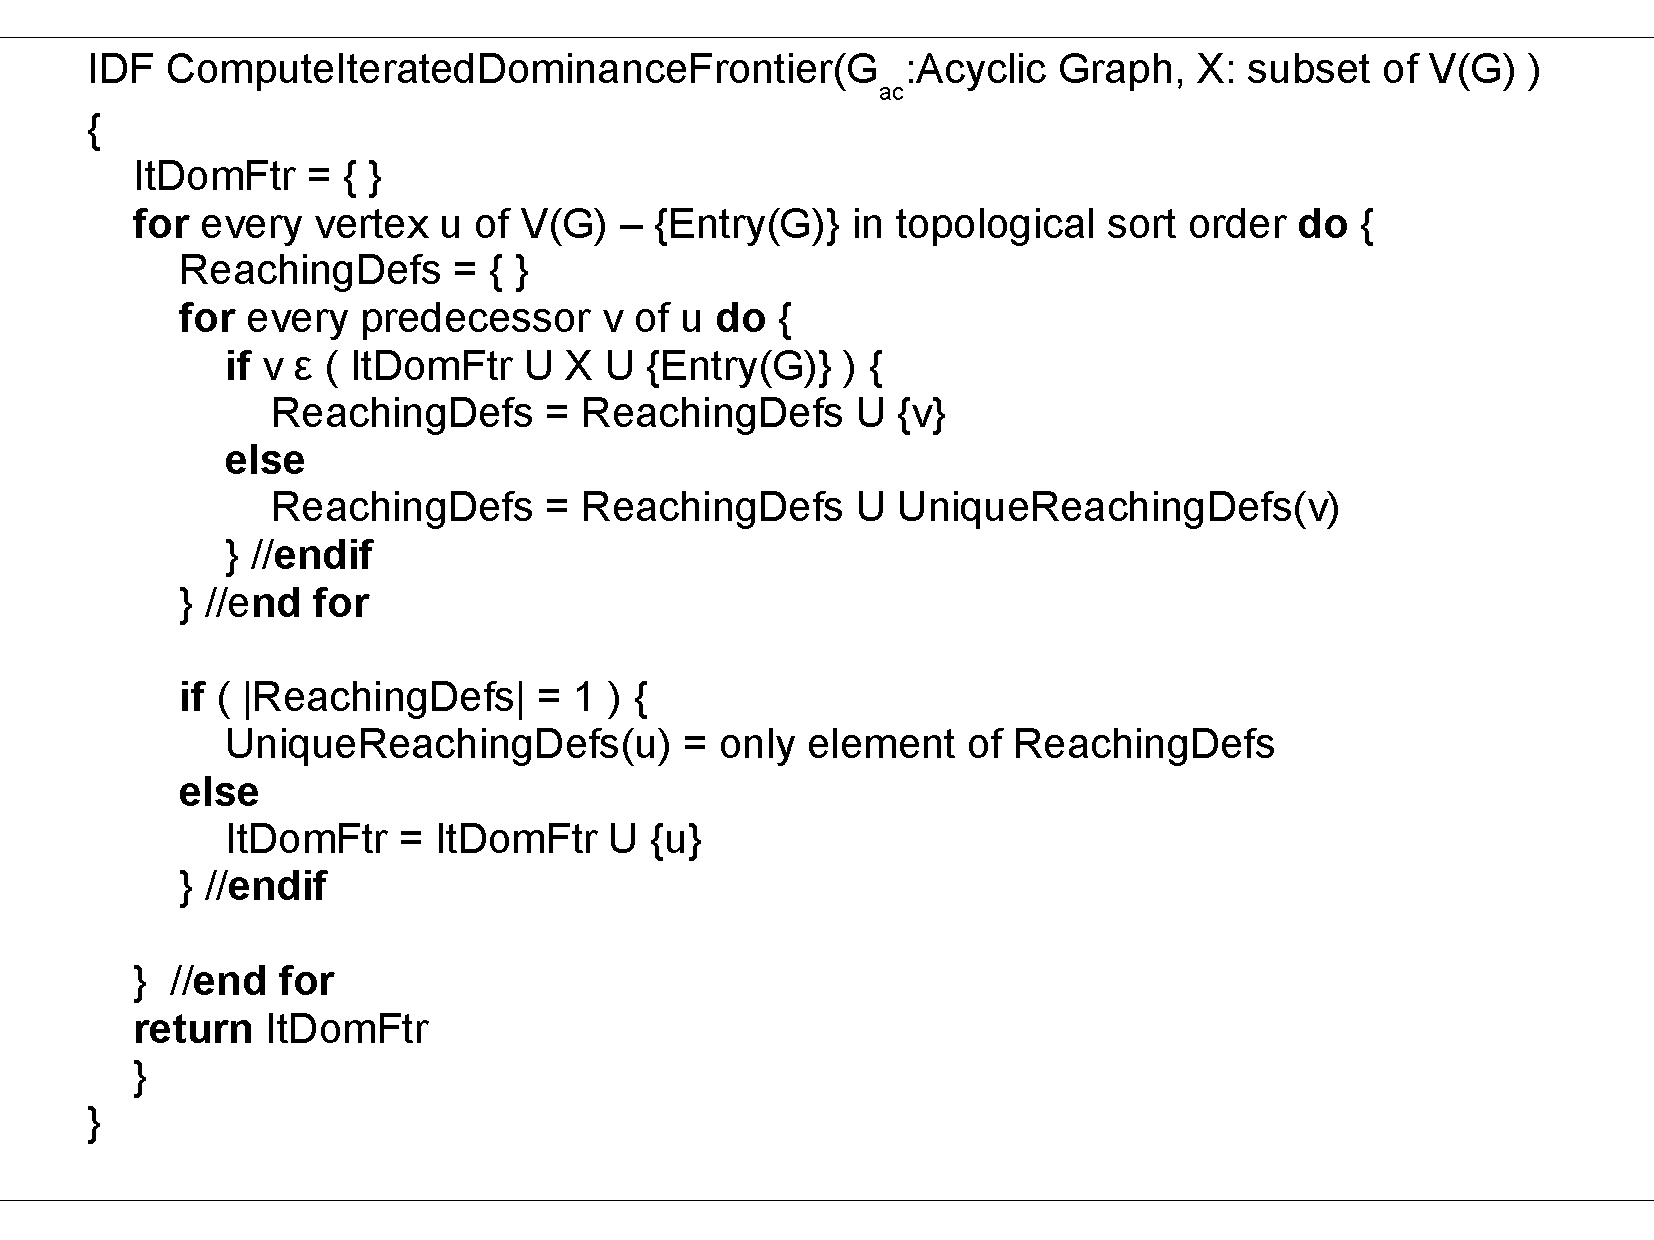
\includegraphics[scale=0.3]{idfcode.pdf}}
%\caption{Pseudocode for computing \iDF of an acyclic graph }
%\label{fig:idfcode}
%\end{figure}  

\begin{algorithm}
  \KwIn{$G_{\textit{fwd}}$: forward CFG}
  \KwIn{$S$: subset of nodes}
  \KwOut{$\iDF(S)$}
  \caption{%ComputeIteratedDominanceFrontier($G_{\textit{fwd}}$, $S$)
  Algorithm for \iDF in an acyclic graph.}
  \label{algo:ramaIDF}

  $\iDF \gets \emptyset$\;
  \lForEach{node $n$}{
    $\textit{UniqueReachingDef}(n) \gets \{\textit{r}\}$
  }
  \ForEach{node $u \neq \textit{r}$ in topological order}{
    $\textit{ReachingDefs} \gets \emptyset$\; 
    \ForEach{$v$ predecessor of $u$}{
      \If{$v \in \iDF \cup S \cup \textit{r}$}{
      $\textit{ReachingDefs} \gets \textit{ReachingDefs} \cup \{v\}$; \label{C:rdf}
      }
      \Else{
      $\textit{ReachingDefs} \gets \textit{ReachingDefs} \cup 
      \textit{UniqueReachingDef}(v)$; \label{C:urdf}
      }
    }
    \If{$|\textit{ReachingDefs}| = 1$}{  \label{C:onerd}
      $\textit{UniqueReachingDef}(u) \gets \textit{ReachingDefs}$; 
    }
    \Else{
      $\iDF \gets \iDF \cup \{u\}$; \label{C:ridf}
    }
  } 
  \Return{$\iDF$}   
\end{algorithm}

Let us walk through this algorithm computing \iDF for variable $v$, i.e., $S = \{4,5,7,12\}$. 
The nodes in Figure~\ref{fig:lnf} are already numbered in topological order. 
Nodes~1 to~5 have only one predecessor, none of them being in $S$, so their \textit{UniqueReachingDef} stays \textit{r}, and \iDF is still empty. 
For node~6, its two predecessors belong to $S$, hence $\textit{ReachingDefs} = \{4,5\}$, and 6 is added to \iDF. 
Nothing changes for 7, then for 8 its predecessors 6 and 7 are respectively in \iDF and $S$: 
they are added to \textit{ReachingDefs}, and 8 is then added to \iDF. 
Finally, for nodes 8 to 12, their \textit{UniqueReachingDef} will be updated to node~8, but this will not change \iDF anymore which will end up being $\{6,8\}$.

\paragraph{\iDF on reducible graphs}
%FAB: ad some details about loops headers, back-edges (using standard notations)...

{\def\HLC{\mbox{HLC}} A reducible graph can be decomposed into an acyclic graph and a set of back-edges. 
  The contribution of back-edges to the iterated dominance frontier can be identified by using the loop nesting forest. 
  If a vertex $v$ is contained in a loop, then $\iDF(v)$ will contain the loop header, i.e. the unique entry of the reducible loop. 
  For any vertex $v$, let $\HLC(v)$ denote the set of loop headers of the loops containing $v$.
  Given a set of vertices $S$, it turns out that $\iDF(S) = \HLC(S) \cup \iDFfwd(S \cup \HLC(S))$ where $\HLC(S)=\bigcup_{v\in S} \HLC(v)$, and where $\iDFfwd$ denote the \iDF restricted to the forward CFG $G_{\textit{fwd}}$.

  Reverting back to Figure~\ref{fig:lnf}, we see that in order to find the $\iDF$ for the nodes defining $x$, we need to evaluate $\iDFfwd(\{4,5,7,12\} \cup \HLC(\{4,5,7,12\}))$. 
  As all these nodes are contained in a single loop with header $2$, $\HLC(\{4,5,7,12\}) = \{2\}$. 
  Computing $\iDFfwd(\{4,5,7,12\})$ gives us $\{6,8\}$, and finally, $\iDF(\{4,5,7,12\}) = \{2,6,8\}$. 
}

\paragraph{\iDF on irreducible graphs}

%\noindent
\begin{figure}[t]
  % \centerline{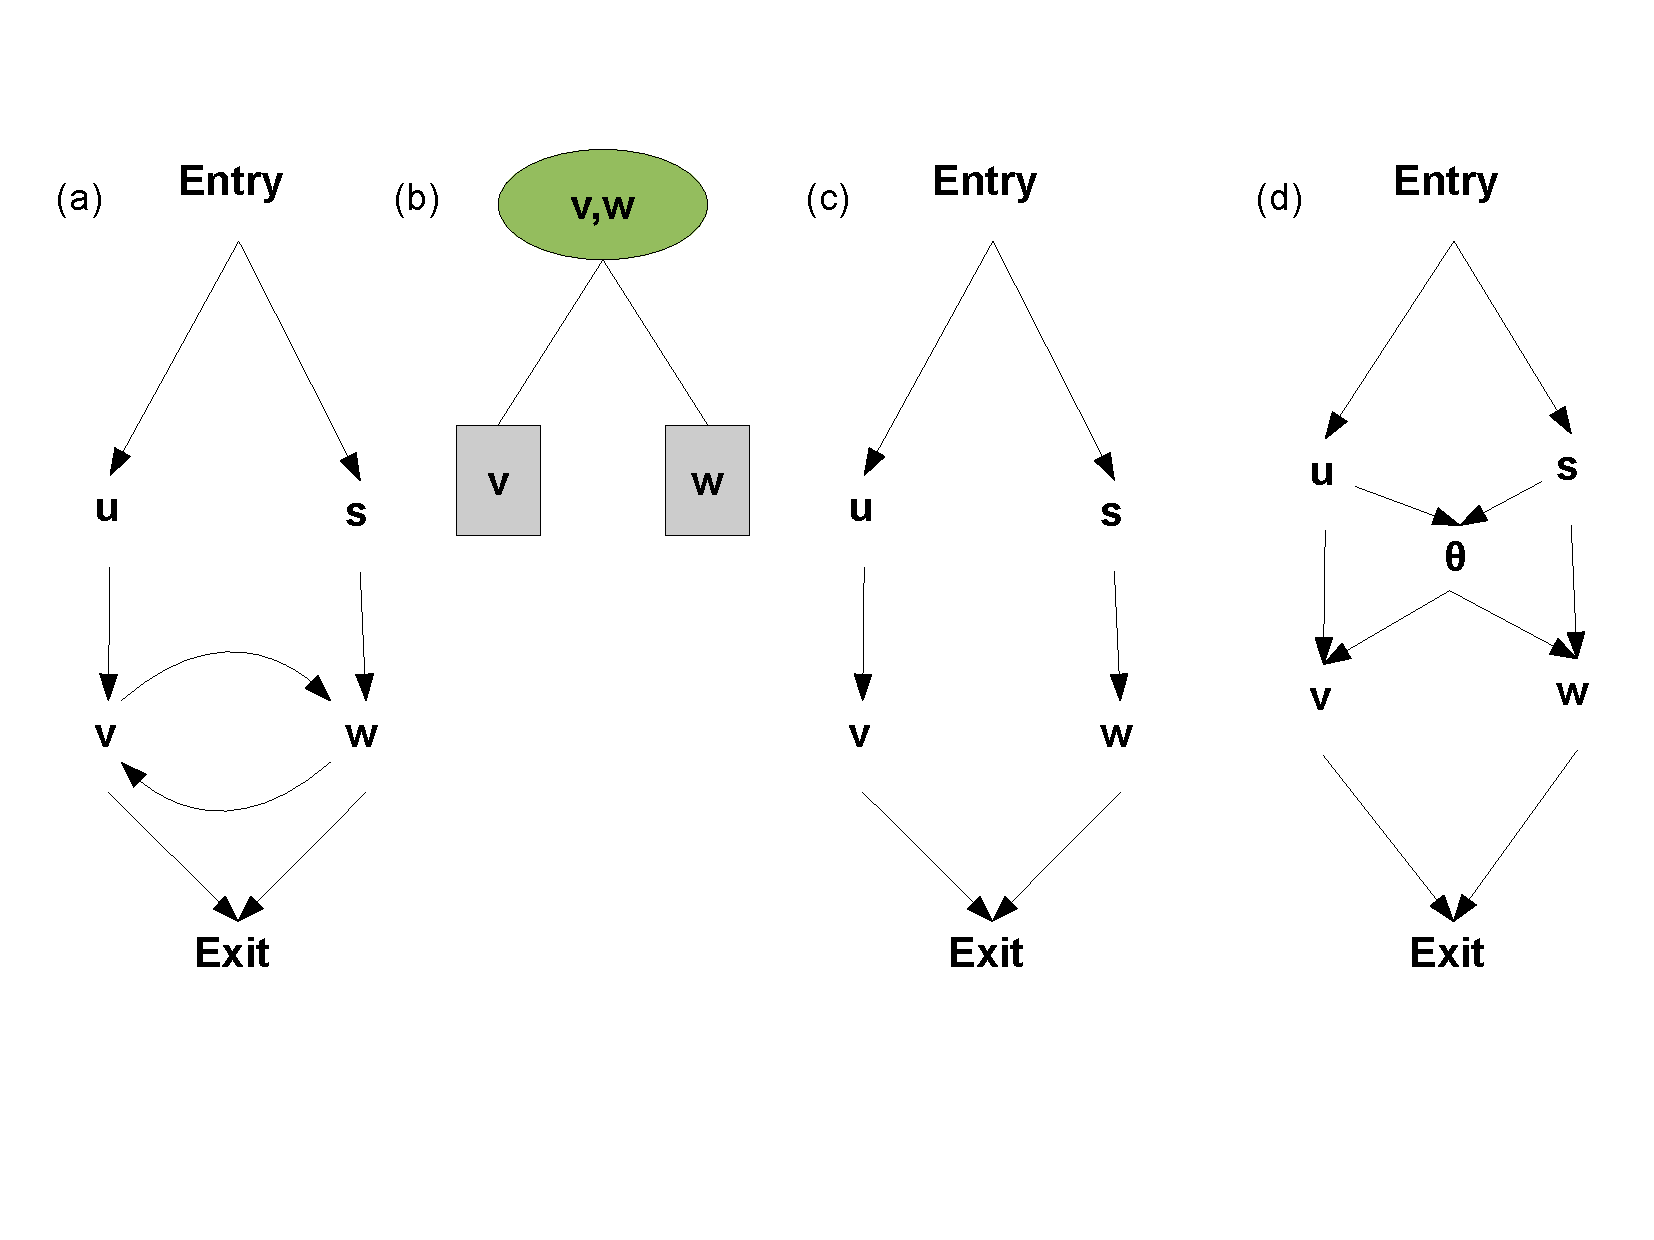
\includegraphics[scale=0.3]{irred.pdf}}
  \subfloat[]{
    \label{sub:alt:irred}
    \tikzsubfigure[1]{irred}
  }
  \hfill
  \subfloat[]{
    \tikzfigure{irred-lnf}
    \label{sub:alt:irred-lnf}
  }
  \hfill
  \subfloat[]{
    \tikzsubfigure[2]{irred}
    \label{sub:alt:irred-acyclic}
  }
  \hfill
  \subfloat[]{
    \tikzsubfigure[3]{irred}
    \label{sub:alt:irred-transf}
  }
  \caption{(a) An irreducible graph (b) The Loop Nesting Forest (c) The acyclic 
    subgraph (d) Transformed graph.}
  \label{fig:irred}
\end{figure} 



We will now briefly explain how graphs containing irreducible loops can be handled. 
The insight behind the implementation is to transform the irreducible loop in such a way that an acyclic graph is created from the loop without changing the dominance properties of the nodes.

\todo{subfigure}
The loop in the graph of Figure~\ref{sub:alt:irred}, that is made up of nodes 
$v$ and $w$, is irreducible as it has two entry nodes, $v$ and $w$.
We let the headers be those entry nodes.
It can be transformed to the acyclic graph \subref{sub:alt:irred-acyclic} by 
removing the back-edges, i.e.  the edges within the loop that point to the 
header nodes, in other words edges $v\rightarrow w$ and $w\rightarrow v$.  We 
create a dummy node, $\theta$, to which we connect all predecessors of the 
headers ($u$ and $s$), and that we connect to all the headers of the loop ($v$ 
and $w$), creating graph \subref{sub:alt:irred-transf}.

Following this transformation, the graph is now acyclic, and computing the \iDF for the nodes in the original irreducible graph translates to computing \iDF using the transformed graph to get $\iDFfwd$ and using the loop forest of the original graph \subref{sub:alt:irred-lnf}.

The crucial observation that allows this transformation to create an equivalent acyclic graph is the fact that the dominator tree of the transformed graph remains identical to the original graph containing an irreducible cycle. 
%FAB: removed the mention of the explosion that was incorrect

\section{Concluding Remarks}

Although all these algorithms claim to be better than the original algorithm by Cytron et al., they are difficult to compare due to the unavailability of these algorithms in a common compiler framework. 

In particular, while constructing the whole \iDF set seems very costly in the classical construction algorithm, its cost is actually amortized as it will serve to place \phifuns for many variables.
It is however interesting not to pay this cost whenever we only have a few variables to consider, for instance when repairing SSA as in the next chapter.
 
Note also that people have observed in production compilers that, during SSA construction, what seems to be the most expensive part is the renaming of the variables and not the placement of \phifuns.



\section{Further Reading}

Cytron's approach for $\phi$-placement involves a fully eager approach of 
constructing the entire \DF-graph \cite{Cytron}.
Sreedhar and Gao proposed the first algorithm for computing \iDF sets without 
the need for explicitly computing the full \DF set \cite{Sreedhar:1995:PoPL}, 
producing the linear algorithm that uses DJ-graphs.

The lazy algorithm presented in this chapter that uses DJ-graph was introduced 
by Sreedhar and Gao and constructs \DF on-the-fly only when a query is 
encountered Pingali and Bilardi \cite{Bilardi1996} suggested a middle-ground by 
combining both approaches.  They proposed a new representation called ADT 
(Augmented Dominator Tree).  The ADT representation can be thought as 
a \DJ-graph, where the \DF sets are pre-computed for certain nodes called 
``boundary nodes'' using an eager approach.  For the rest of the nodes, termed 
``interior nodes,'' the \DF needs to be computed on-the-fly as in the 
Sreedhar-Gao algorithm.  The nodes which act as ``boundary nodes'' are detected 
in a separate pass.  A factor $\beta$ is used to determine the partitioning of 
the nodes of a CFG into boundary or interior nodes by dividing the CFG into 
zones.  $\beta$ is a number that represents space/query-time tradeoff.  $\beta 
<\!\!< 1$ denotes a fully eager approach where storage requirement for \DF is 
maximum but query-time is faster while $\beta >\!\!> 1$ denotes a fully lazy 
approach where storage requirement is zero but query is slower.

Given the ADT of a control-flow graph, it is straight forward to modify Sreedhar and Gao's algorithm for computing \phifuns in linear time. 
The only modification that is needed is to ensure that we need not visit all the nodes of a sub-tree rooted at a node $y$ when $y$ is a boundary node whose \DF set is already known. 
This change is reflected in Line \ref{C:cached} of Algorithm~\ref{algo:IDFMain}, where a subtree rooted at $y$ is visited or not visited based on whether it is a boundary node or not.

The algorithm computing \iDF without the explicit \DF-graph is from Das \& 
Ramakrishna \cite{Das-Rama:2005}.
For iterative \iDF set computation, they also exhibit TDMSC-II, an improvement 
to algorithm TDMSC-I.  This improvement is fueled by the observation that for 
an inconsistent node $u$, the \iDF sets of all nodes $w$ such that $w$ 
dominates $u$ and $w.\depth \geq u.\depth$, can be locally corrected for some 
special cases.  This heuristic works very well for certain class of 
problems---especially for CFGs with \DF-graphs having cycles consisting of 
a few edges.  This eliminates extra passes as an inconsistent node is made 
consistent immediately on being detected.

Finally, the part on computing \iDF sets using loop nesting forests is based on 
Ramalingam's work on loops, dominators, and dominance frontiers 
\cite{ramalingam:loopforest}.

% \paragraph{TODO: citations}
% \begin{itemize}
  % \item SSA form \cite{cfr}
  % \item Sreedhar \& gao \cite{sreedhar_popl}
  % \item Das \& Ramakrishna no explicit \DF-graph construction  \cite{das}
% \end{itemize}
% }
